\chapter{软件系统与操作流程}

密码原语解决具体数学问题，软件系统还要负责组合选择、参数检查、对象保存和用户操作。本章
介绍系统怎样把后端、公共协议和应用入口分开，以及新增HIBE或IBS时需要完成哪些工作。

\section{分层软件架构}

系统自下而上分为基础设施层、密码原语层、组合层、协议层和应用层。基础设施层提供规范编码、
随机源、域分隔哈希、错误类型和原子文件保存。密码原语层分别实现HIBE和IBS。组合层根据配置
选择后端，并在生成密钥前完成能力与容量检查。协议层实现第三章的五个IB-ME算法。最上层提供
命令行、实验工具和浏览器演示。

\begin{figure}[H]
\centering
\begin{tikzpicture}[node distance=7mm and 8mm]
 \node[flow,text width=92mm] (web) {应用层：浏览器、CLI、实验工具};
 \node[flow,below=of web,text width=92mm] (protocol) {协议层：IB-ME五算法、Hybrid、字节认证};
 \node[check,below=of protocol,xshift=-27mm,text width=38mm] (assembly) {组合层\\SuiteConfig、注册表、预检};
 \node[check,below=of protocol,xshift=27mm,text width=38mm] (state) {状态层\\固定发钥、对象保存、恢复};
 \node[flow,below=of assembly,text width=38mm] (hibe) {HIBE后端\\LATTE、Lai};
 \node[flow,below=of state,text width=38mm] (ibs) {IBS后端\\六种签名实现};
 \node[check,below=of protocol,yshift=-48mm,text width=92mm] (core) {基础设施：规范编码、随机源、哈希、错误处理};
 \draw[flowarrow](web)--(protocol);
 \draw[flowarrow](protocol)--(assembly);
 \draw[flowarrow](protocol)--(state);
 \draw[flowarrow](assembly)--(hibe);
 \draw[flowarrow](state)--(ibs);
 \draw[flowarrow](hibe)--(core);
 \draw[flowarrow](ibs)--(core);
\end{tikzpicture}
\caption{软件系统的分层结构}
\label{fig:system-structure}
\end{figure}

这一结构有两个直接作用。第一，公共协议不根据算法名称编写分支。它只调用接口，并从组合配置
读取容量和格式。第二，应用入口不直接操作陷门、矩阵或多项式；命令行和浏览器收到的都是统一
角色对象和密文字节。因此，同一套页面、状态管理和错误处理可以服务不同组合。

\section{稳定的原语接口}

HIBE后端提供五个密码方法，IBS后端提供四个密码方法和一个签名加载方法。表
~\ref{tab:backend-interfaces}列出接口及其返回对象。

\begin{table}[H]
\centering\small
\caption{HIBE与IBS后端接口}
\label{tab:backend-interfaces}
\begin{tabularx}{\textwidth}{@{}p{.16\textwidth}p{.2\textwidth}X@{}}
\toprule
\rowcolor{black!8} 后端 & 方法 & 公共含义 \\
\midrule
HIBE & $\mathsf{setup}$ & 建立公开参数与主秘密 \\
HIBE & $\mathsf{extract}$ & 为第一层接收身份生成密钥 \\
HIBE & $\mathsf{derive}$ & 为第二层发送身份委派叶密钥 \\
HIBE & $\mathsf{encrypt}$ & 沿两层身份路径加密固定长度种子 \\
HIBE & $\mathsf{decrypt}$ & 用叶密钥恢复种子或返回拒绝 \\
\midrule
IBS & $\mathsf{setup}$ & 建立签名公开参数与主秘密 \\
IBS & $\mathsf{key\_extract}$ & 为发送身份生成签名密钥 \\
IBS & $\mathsf{sign}$ & 签署规范协议消息 \\
IBS & $\mathsf{verify}$ & 以公开参数、身份和消息验签 \\
IBS & $\mathsf{load\_signature}$ & 从规范字节恢复签名对象 \\
\bottomrule
\end{tabularx}
\end{table}

每种公开参数、主秘密、用户密钥、密文和签名都实现规范的$\mathsf{to\_bytes}$与
$\mathsf{from\_bytes}$。对象头包含类别、版本和参数摘要。后端加载对象时检查字段数量、长度、
数值范围和公开上下文，公共层无需了解其中的系数排列。

接口也明确随机源的传递方式。建立、发钥、加密和随机化签名从上层取得密码学随机源；验签与
规范解码不读取随机数。测试可以注入可重复随机流，正常运行使用操作系统随机源。同一方法在
不同入口下因此保持相同的随机性边界。

\section{组合配置与接入流程}

\subsection{完整组合配置SuiteConfig}

一套运行配置由$\mathsf{SuiteConfig}$描述。它记录HIBE与IBS选择器、算法版本、两边参数档、
密钥和签名格式、外部身份长度、混合载荷预算以及协议版本。配置使用排序字段和规范JSON编码，
其摘要进入公开对象和所有角色密钥。

注册表为每个后端保存四类信息：构造函数、参数预设、对象解码器和能力声明。能力声明包括
两层身份支持、内部身份宽度、直接明文容量、IBS输入上限、签名尺寸上界、所需运行依赖和允许的
编码格式。发现后端和查看配置只读取这些静态信息，不生成密钥。

运行前的$\mathsf{validate\_suite}$依次完成：
\begin{enumerate}
  \item 解析HIBE与IBS选择器，固定精确版本和参数档；
  \item 检查HIBE支持两层身份，外部身份编码后不超过内部上限；
  \item 计算IBS签名输入开销和最大应用消息长度；
  \item 检查签名上界与应用消息能够放入混合载荷预算；
  \item 检查对象格式和运行依赖，生成完整配置摘要。
\end{enumerate}
只有配置通过以后，系统才进入$\mathsf{Setup}$。容量不足会在昂贵建立之前给出所需字节数和
现有预算，用户可以选择更大载荷预算或另一后端。

\subsection{新增HIBE或IBS的接入步骤}

接入新HIBE时，实现者完成五个HIBE方法和五类对象，声明两层身份宽度、种子容量和参数预设，
再向注册表提供一个后端描述。接入新IBS时，实现四个密码方法、签名加载和四类对象，声明身份、
签名输入及签名输出上限。公共协议、Hybrid、BYTEAUTH、状态文件和应用入口均不修改。

\begin{figure}[H]
\centering
\begin{tikzpicture}[node distance=7mm and 7mm]
 \node[flow,text width=36mm] (alg) {实现论文算法\\与严格对象};
 \node[flow,right=of alg,text width=36mm] (cap) {声明参数、容量\\和编码格式};
 \node[flow,right=of cap,text width=36mm] (reg) {注册BackendSpec\\获得SuiteConfig};
 \node[check,below=of cap,text width=38mm] (unit) {原语正例、错身份\\篡改与恢复测试};
 \node[check,left=of unit,text width=38mm] (combo) {与现有另一类原语\\完成组合测试};
 \node[check,right=of unit,text width=38mm] (app) {沿用CLI与Web\\完成实际收发};
 \draw[flowarrow](alg)--(cap);
 \draw[flowarrow](cap)--(reg);
 \draw[flowarrow](reg)--(unit);
 \draw[flowarrow](unit)--(combo);
 \draw[flowarrow](unit)--(app);
\end{tikzpicture}
\caption{新增密码后端的接入过程}
\label{fig:new-backend}
\end{figure}

以Wang--PW为例，新增代码位于独立IBS目录，向外暴露与Sageloli、SRGG相同的方法。注册描述声明
目标档$s0$-4、393,320字节签名和4,096字节签名输入上限。组合层据此算出3,924字节应用容量，
并把混合载荷预算提高到能够容纳该签名的范围。随后直接复用LATTE、五个IB-ME算法、命令行角色
导入和错误输入流程；公共协议仍使用统一接口和处理顺序，不增加后端专属分支。

这一接入方式也是“通用设计”的软件依据。更换算法需要完成新原语本身及其元数据，而不是复制
一套IB-ME实现。十种常规配对和LATTE＋Wang--PW都经过同一入口形成。

\section{固定发钥与持久状态}

现实系统不会为每条消息重新建立主密钥。发钥机构需要长期保存主状态，并保证同一身份能够取回
先前发布的密钥。作品为HIBE接收者和IBS发送者分别维护发钥记录。

一次发钥分为准备、生成和提交三个阶段。准备阶段取得本地锁并写入待处理身份；生成阶段调用
底层原语；提交阶段先原子保存更新后的主状态，再发布用户密钥。若进程在生成中断，恢复程序会
看到待处理记录并停止继续发钥，避免同一身份在状态不明时获得第二份对象。

加载状态时，系统按图~\ref{fig:state-recovery}检查组合配置、公开上下文、参数快照、对象类型和
身份绑定。后端随后检查自己的代数关系，例如LATTE叶钥方程、SRGG对象形状或Wang--PW的
$AX+H_1=G$关系。通过后才恢复运行实例。

\begin{figure}[H]
\centering
\begin{tikzpicture}[node distance=8mm and 8mm]
 \node[flow,text width=34mm] (files) {读取公开对象\\主状态与角色密钥};
 \node[flow,right=of files,text width=34mm] (codec) {规范解码\\版本与长度检查};
 \node[flow,right=of codec,text width=34mm] (bind) {配置摘要、身份\\公开参数绑定};
 \node[check,below=of codec,text width=40mm] (math) {后端代数关系与状态账本检查};
 \node[check,left=of math,text width=36mm] (runtime) {恢复运行实例\\继续加密或解密};
 \draw[flowarrow](files)--(codec);
 \draw[flowarrow](codec)--(bind);
 \draw[flowarrow](bind)--(math);
 \draw[flowarrow](math)--(runtime);
\end{tikzpicture}
\caption{持久对象恢复流程}
\label{fig:state-recovery}
\end{figure}

公开对象、发送密钥、接收密钥和密文可以分别导出。角色导入只要求该角色实际需要的对象：
发送端不读取HIBE主秘密，接收端不读取IBS主秘密。这样可以在不同进程甚至不同主机上执行发送
和接收，同时保持相同的组合配置与编码。

\section{命令行与浏览器操作}

命令行适合批量实验、持久状态和跨进程恢复。典型流程为：选择组合并建立系统；为Alice、Bob
导出角色密钥；Alice指定Bob并加密；Bob指定Alice并解密；关闭进程后重新导入对象，再次解密
已有密文。实验驱动在此基础上记录每阶段时间、对象字节数和进程树RSS。

浏览器界面使用同一运行时，不另写一套密码代码。使用者首先选择组合，然后输入接收者、发送者、
期望发送者和消息。页面显示建立、发钥、签名、封装和解密阶段，并展示密文长度、耗时和最终
结果。对于耗时较长的B组，任务在服务端继续执行，页面刷新后可以重新连接正在运行的任务。

\begin{figure}[H]
\centering
\includegraphics[width=.98\textwidth]{../../deliveries/2026-10-20-web-redesign/desktop.png}
\caption{A组实际收发界面：指定双方身份、加密消息与匹配解密}
\label{fig:web-demo}
\end{figure}

图~\ref{fig:web-demo}记录A组的一次实际操作：Alice向Bob发送36字节UTF-8消息，Bob选择Alice为
期望发送者后恢复原文。A、B还分别在同一条密文上执行三种身份错配、翻转1 bit和截短1字节，
均得到拒绝。两组该次密文长度分别为142,095字节和149,255字节。

\begin{figure}[H]
\centering
\begin{minipage}[t]{.49\textwidth}
\centering
\includegraphics[width=\linewidth,trim=420 320 130 180,clip]{../../deliveries/2026-10-20-web-redesign/desktop.png}
\par\smallskip\textbf{（a）身份匹配并恢复原文}
\end{minipage}\hfill
\begin{minipage}[t]{.49\textwidth}
\centering
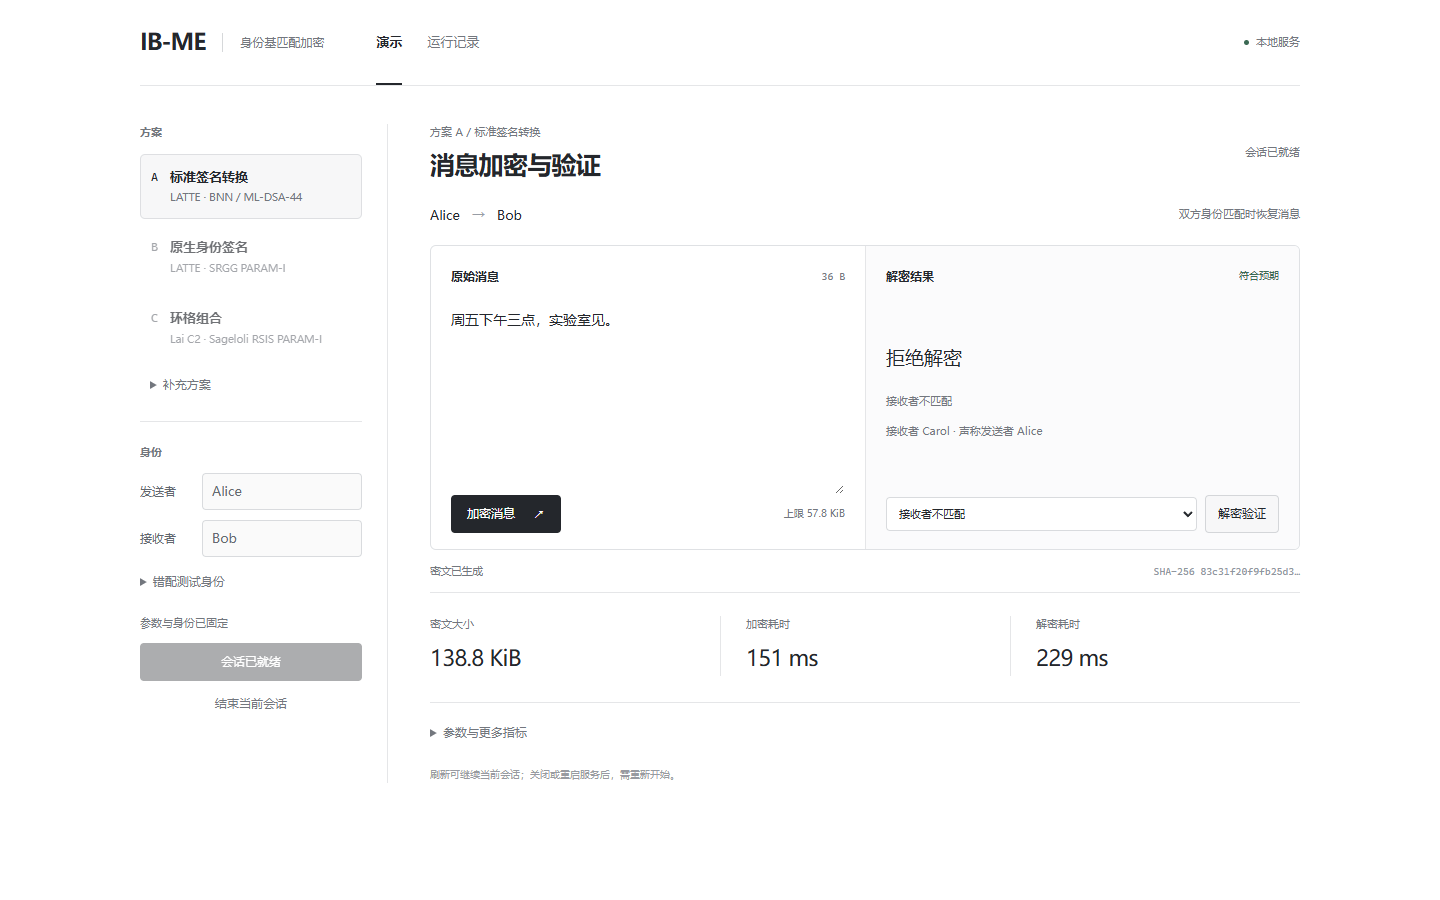
\includegraphics[width=\linewidth,trim=420 320 130 180,clip]{../../deliveries/2026-10-20-web-rejection-screenshots/wrong-receiver.png}
\par\smallskip\textbf{（b）接收身份不匹配并拒绝}
\end{minipage}
\caption{网页演示关键结果局部：发送者、接收者、期望发送者与解密结果}
\label{fig:web-demo-details}
\end{figure}

\section{运行优化与部署方式}

除了第五章的三项主要优化，系统还减少两类重复工作。BNN签名包含机构证书和用户消息签名。对
同一身份的连续消息，系统缓存“证书已经验证”的公开结果，但每条消息仍重新验证用户签名。
缓存绑定完整证书、用户公钥和身份，并使用有界LRU管理。

SRGG签名的一部分数值准备只取决于固定签名密钥和数值选项。实现可以复用该计划，每条签名仍
重新生成随机量。实验表明这两类局部缓存对完整流程的影响小于结构化采样、紧凑编码和Lai会话，
因此它们作为运行细节保留。

系统支持单机演示和分角色部署。单机模式把发钥机构、发送端、接收端和浏览器服务放在一台主机，
便于比赛现场操作。分角色模式由发钥机构离线生成角色对象，发送端和接收端分别导入自己的密钥；
密文可通过任意字节传输通道送达。

\begin{figure}[H]
\centering
\begin{tikzpicture}[node distance=9mm and 12mm]
 \node[check,text width=38mm] (issuer) {发钥机构\\建立系统、签发角色密钥};
 \node[flow,below left=of issuer,text width=36mm] (sender) {发送端\\导入公开对象与发送密钥};
 \node[flow,below right=of issuer,text width=36mm] (receiver) {接收端\\导入公开对象与接收密钥};
 \node[check,below=of issuer,yshift=-34mm,text width=38mm] (channel) {公开传输通道\\只传递规范密文};
 \draw[flowarrow](issuer)--node[left,font=\small]{发送角色对象}(sender);
 \draw[flowarrow](issuer)--node[right,font=\small]{接收角色对象}(receiver);
 \draw[flowarrow](sender)--(channel);
 \draw[flowarrow](channel)--(receiver);
\end{tikzpicture}
\caption{发钥机构、发送端与接收端的部署关系}
\label{fig:deployment}
\end{figure}

原生模块在创建适配器时会检查接口和二进制。已有部署对照发现，把安装包和运行文件放在Linux
本地文件系统可以减少跨挂载目录的重复读取。该调整不改变算法、参数和密文格式，第七章列出
同一运行时下的对照结果。

除主要实验机器外，项目还在Xeon Silver 4216主机的NixOS、Sage~10.9和Python~3.14.7环境
完成独立安装。A、B各执行25条操作，C完成匹配解密、内部签名拒绝和恢复。C最初因900秒阶段上限导致超时；
调整为3600秒后完成三个长阶段，耗时约21至27分钟。这次复现用于检查安装、对象恢复和完整调用路径；
性能分析仍采用第七章逐项列明的原始实验环境。

\section{本章小结}

软件系统通过稳定接口、组合配置和注册表把底层算法与公共协议分开。新增后端只实现自身算法、
对象与能力声明，随后即可复用五个IB-ME算法、状态管理、CLI和浏览器入口。固定发钥和规范恢复
使系统能够跨进程长期使用，单机与分角色部署则覆盖演示和实际通信两种方式。
